\documentclass{beamer}
\usetheme{Boadilla}

\usepackage{amsmath}
\usepackage{amsfonts}
\usepackage{hyperref}
\usepackage{xcolor}

\usepackage{amsmath}
\DeclareMathOperator*{\argmax}{arg\,max}
\DeclareMathOperator*{\argmin}{arg\,min}

\title{AutoML-Zero: Evolving Machine Learning Algorithms From Scratch}
\author{Kseniia Petrushina}
\institute{MIPT, 2024}


\begin{document}

\begin{frame}
    \titlepage
\end{frame}


\begin{frame}
    \tableofcontents
\end{frame}


\section{Motivation}
\begin{frame}{Motivation}
    \begin{block}{AutoML}
        Automate the design of model structures and learning methods
    \end{block}
    
    \begin{block}{Current solutions}
        \begin{itemize}
            \item Growing networks neuron-by-neuron
            \item Bayesian hyperparameter optimization
            \item Neural architecture search (including fine-grained search)
            \item Joint neural architecture and hyperparameter search
        \end{itemize}
    \end{block}

    \begin{block}{Limitations}
        \begin{itemize}
            \item Human bias due to the creation of building blocks
            \item Limited search space
        \end{itemize}
    \end{block}
\end{frame}


\section{Algorithm}

\begin{frame}{Proposed approach}
    \begin{block}{Idea}
        Evolutionary symbolic search over basic mathematical operations
    \end{block}

    \begin{block}{Process formulation}
    \begin{enumerate}
        \item Given a set of ML tasks $\mathcal{T}$, find optimal algorithm $\alpha^* \in \mathcal{A}$
        \item Quality of $\alpha$ is measured on $\mathcal{T}_{search} \subset \mathcal{T}$. Each search experiment produces candidate algorithm
        \item The best candidate is chosen on $\mathcal{T}_{select} \subset \mathcal{T}$
    \end{enumerate}
        
    \end{block}

    \begin{block}{Search space}
        \begin{itemize}
            \item Functions (\texttt{Setup, Predict, Learn})
            \item Scalar, vector and matrix variables
            \item Instruction with mathematical operation
        \end{itemize}
    \end{block}

\end{frame}

\begin{frame}{Evaluation}
 
    \begin{figure}
        \centering
        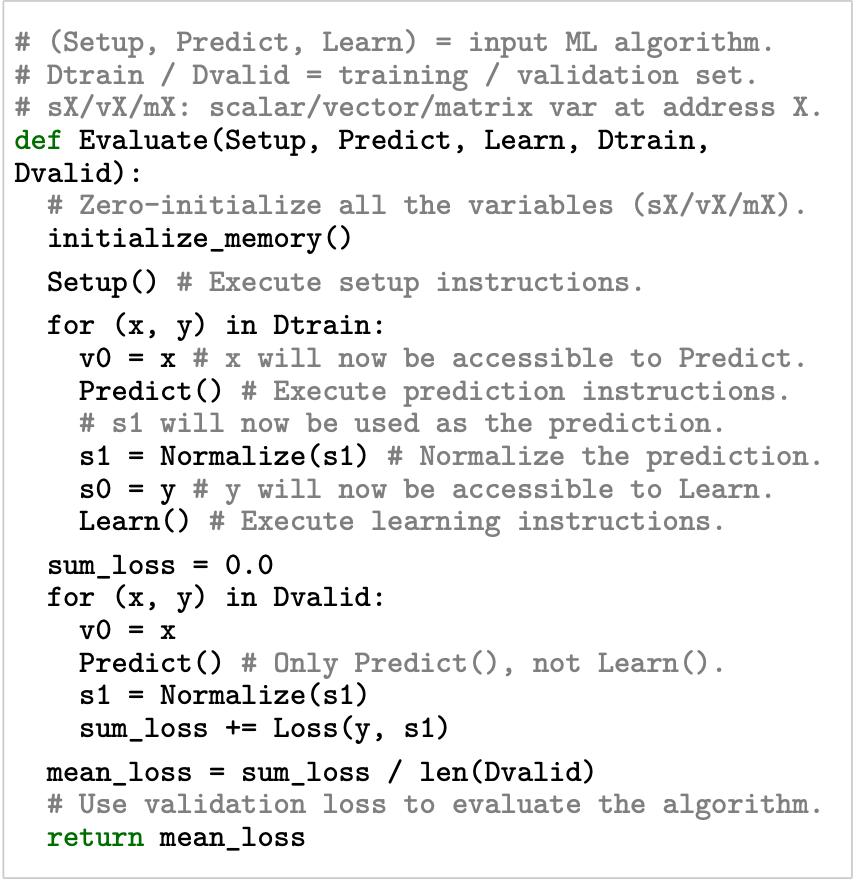
\includegraphics[scale=0.24]{eval.png}
        \caption{Algorithm evaluation on one task.}
        \label{fig:success}
    \end{figure}
    
\end{frame}

\begin{frame}{Evolutionary algorithm}
 
    \begin{figure}
        \centering
        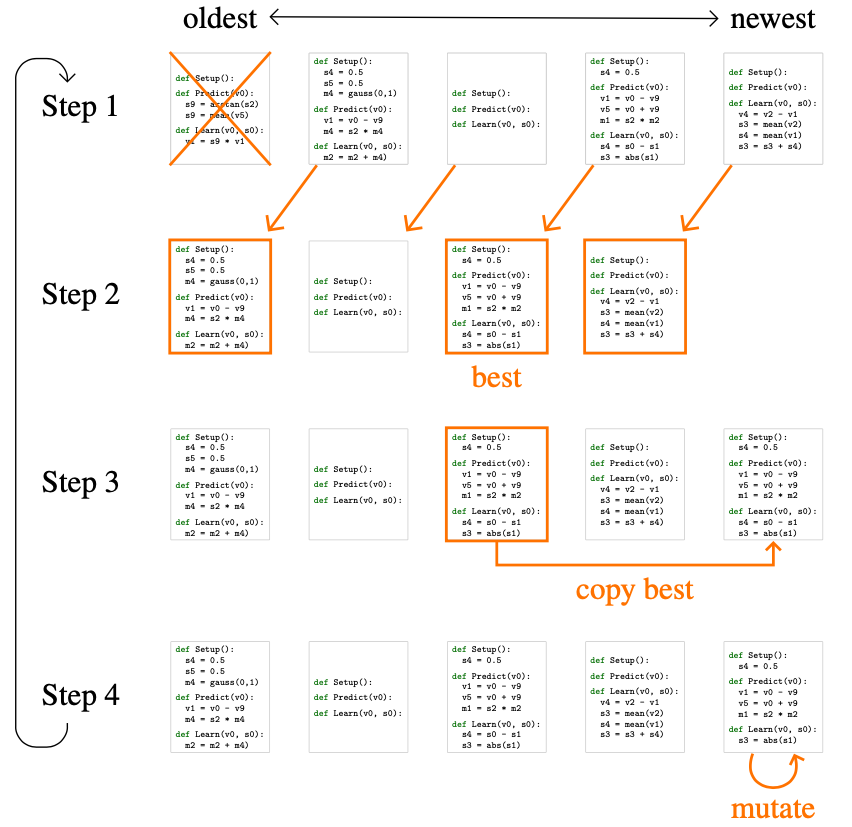
\includegraphics[scale=0.24]{evolution.png}
        \caption{One cycle of the evolutionary method.}
        \label{fig:evol}
    \end{figure}
    
\end{frame}


\begin{frame}{Evolutionary algorithm}
 
    \begin{figure}
        \centering
        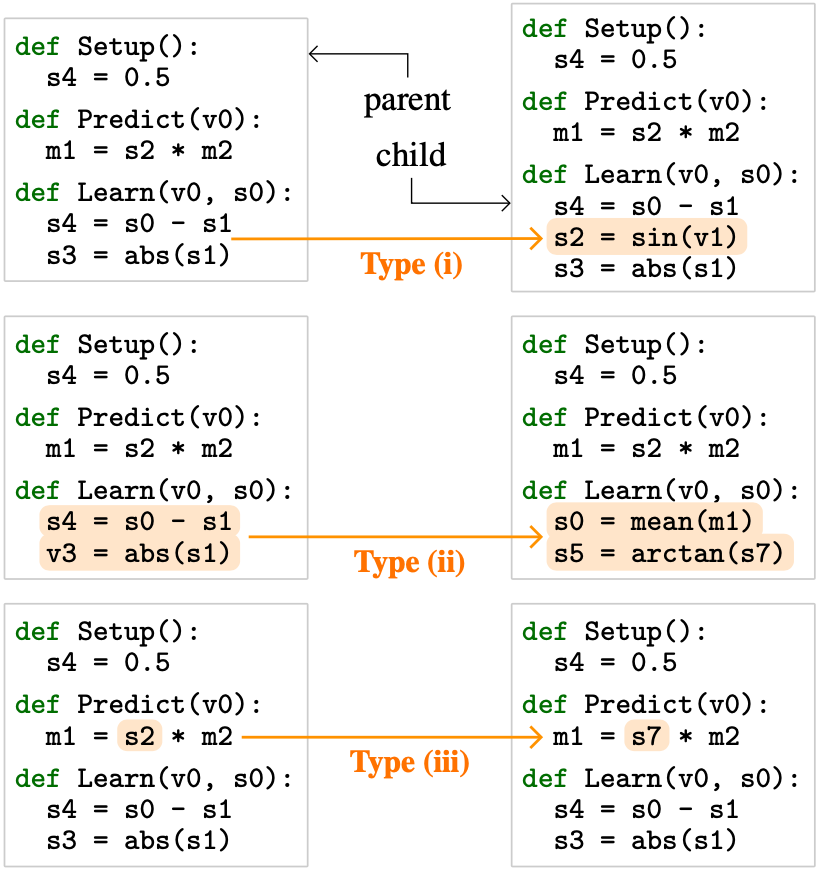
\includegraphics[scale=0.24]{mutation.png}
        \caption{Mutation examples.}
        \label{fig:mut}
    \end{figure}
    
\end{frame}

\section{Results}

\begin{frame}{Results}
 
    \begin{figure}
        \centering
        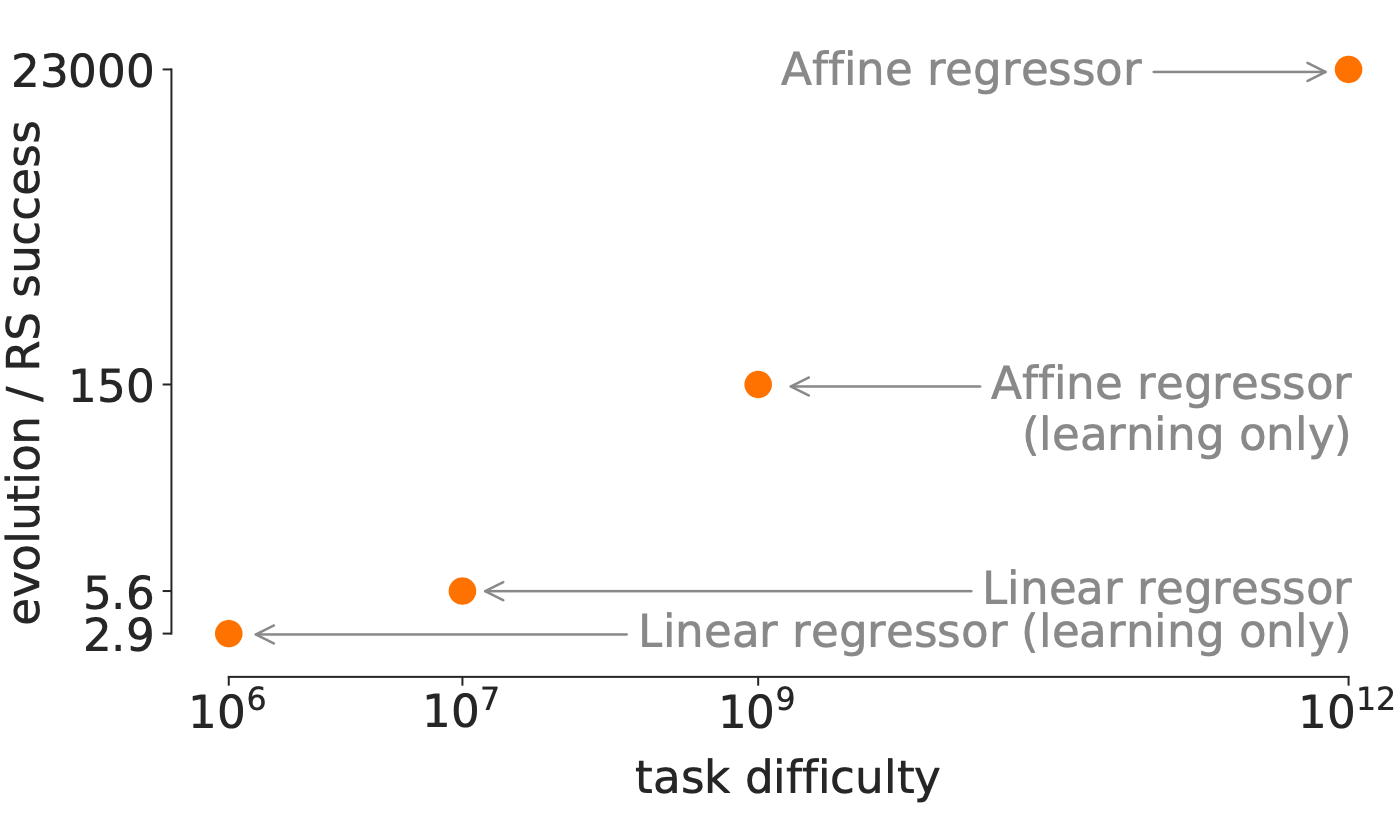
\includegraphics[scale=0.2]{success.png}
        \caption{Relative success rate of evolution and random search (RS).}
        \label{fig:success}
    \end{figure}
    
\end{frame}

\begin{frame}{Results}
\begin{columns}

    \begin{column}{0.48\textwidth}
    
    \begin{block}{Non-linear data}
        \textit{Teacher} neural networks generates regression tasks.

        \begin{itemize}
            \item $\mathcal{T}_{search}$ consists of 1 task - the algorithm hard-codes \textit{teacher} weights
            \item $\mathcal{T}_{search}$ consists of 100 task - evolution discovers the forward pass and “invents” back-propagation code
        \end{itemize}
    
    \end{block}

    \end{column}

    \begin{column}{0.5\textwidth}
        
    
    \begin{figure}
        \centering
        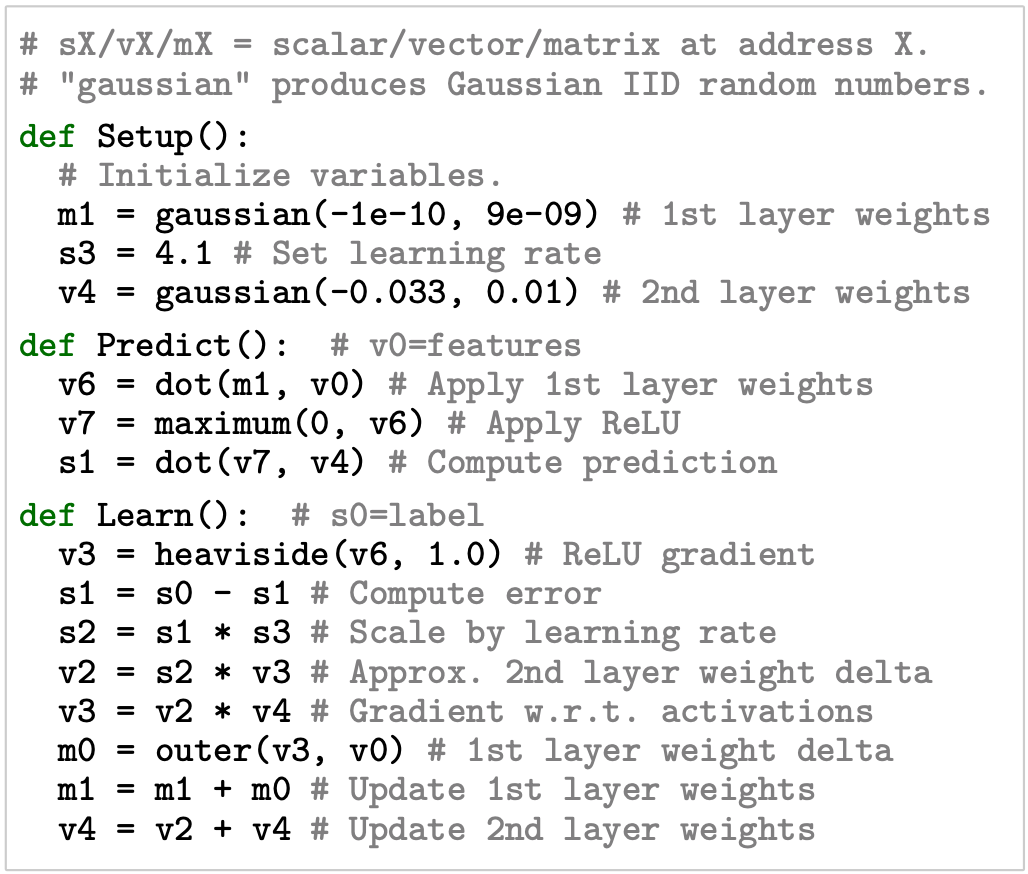
\includegraphics[scale=0.15]{neuralnet.png}
        \caption{Relative success rate of evolution and random search (RS).}
        \label{fig:nn}
    \end{figure}
    \end{column}
\end{columns}
\end{frame}

\begin{frame}{Results}
 
    \begin{figure}
        \centering
        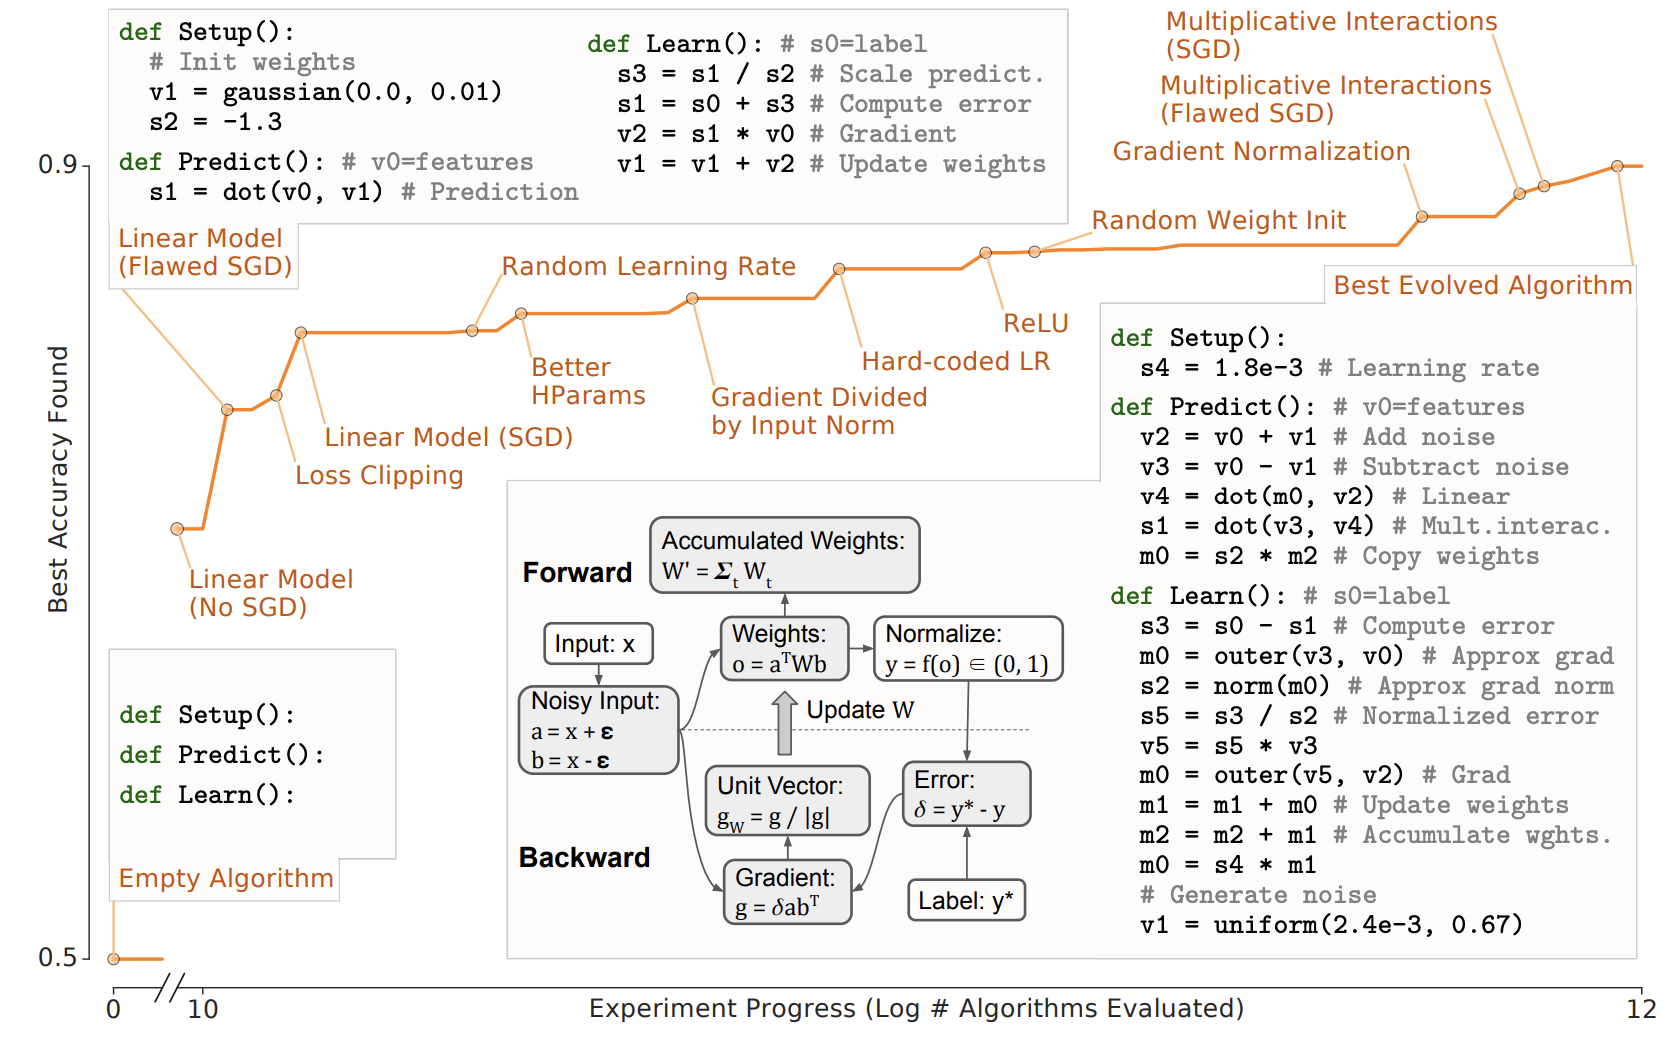
\includegraphics[scale=0.4]{progress.png}
        \caption{Progress of one evolution experiment on projected binary CIFAR-10.}
        \label{fig:prog}
    \end{figure}
    
\end{frame}


\begin{frame}{Results}
 
    \begin{block}{Emerging techniques}
    \begin{itemize}
        \item Regularization
        \[\mathbf{a} = \mathbf{x} + \mathbf{u},\quad \mathbf{b} = \mathbf{x} - \mathbf{u},\quad \mathbf{u} = \mathbf{U}(\alpha, \beta) \]
        \item Multiplicative interactions
        \[\mathbf{o} = \mathbf{a}^T\mathbf{W} \mathbf{b}\]
        \item Gradient normalization
        \[\mathbf{g_w} = \frac{\mathbf{g}}{|\mathbf{g}|}; \quad \mathbf{g} = \delta \mathbf{a} \mathbf{b}^T; \quad \delta = \mathbf{y}^* - \mathbf{y}\]
        \item Weight averaging
        \[\mathbf{W'} = \sum_\mathbf{t} \mathbf{W_t} \]
    \end{itemize}
        
    \end{block}
    
\end{frame}

\begin{frame}{Results}
 
    \begin{figure}
        \centering
        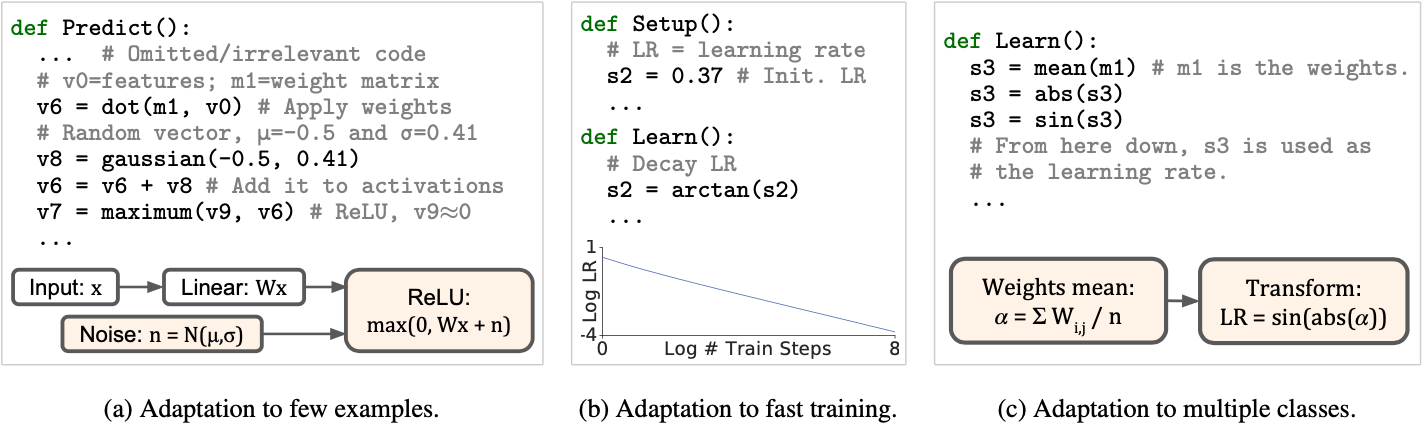
\includegraphics[scale=0.23]{adaptation.png}
        \caption{Adaptations to different task types.}
        \label{fig:adapt}
    \end{figure}
    
\end{frame}

\begin{frame}{Conclusion}
    \begin{block}{Discussion}
        \begin{itemize}
            \item The search method scalability
            \item Evaluating evolved algorithms\\
            \item Interpreting evolved algorithms
            \item Search space enhancements
        \end{itemize}
    \end{block}
\end{frame}

\begin{frame}{Literature}
    \begin{enumerate}
        \item \textbf{Main article} \href{https://proceedings.mlr.press/v119/real20a/real20a.pdf}
        {AutoML-Zero: Evolving Machine Learning Algorithms From Scratch}.
    \end{enumerate}
\end{frame}




\end{document}